\setcounter{section}{5}
\setcounter{subsection}{2}
\setcounter{question}{0}

%%%%%%%%%%%%%%%%%%%%%%%%%%%%%%%%%%%%%%%%%%%%%%%%%%%%%%%%%%%%%%%%%%%%%%%%%%%
% Assignment 5.2: Generating and interpreting z-scores and t-scores
%%%%%%%%%%%%%%%%%%%%%%%%%%%%%%%%%%%%%%%%%%%%%%%%%%%%%%%%%%%%%%%%%%%%%%%%%%%

\rassignment{Assignment 5.2: Generating and interpreting z-scores and t-scores}

In assignment 5.1 you have seen that to calculate a 95\% one-sided \concept{confidence interval} for a \concept{sample} with $n \geq 30$ you need to use the correct \concept{z-value}. Now you are going to find out how to get that number from \texttt{R} using the \rcode{qnorm()} function. The \rcode{qnorm()} function returns the \rcode{x}-value for a certain probability for a specified \concept{normal distribution}, if you do not specify the \concept{mean} (\rcode{mean}) and \concept{standard deviation} (\rcode{sd}) arguments it returns the \concept{z-value} for the \concept{standard normal distribution}. \\

Run the following code in R: \\

\codeblock{qnorm(p = 0.95, mean = 0, sd = 1, lower.tail = TRUE)\\
{\color{dataset} \# Or because the standard normal distribution is the default simply use:}\\
qnorm(0.95)
}

\question{
    Round the number to 3 decimals. Do you recognise this \concept{z-value}?
}

\emptyanswerbox{
    Result: \shortanswerline
    \answerskip
    \rule{\textwidth}{0.4pt}
}

In assignment 5.1 you have also seen that for the 95\% two-sided \concept{confidence interval} for a \concept{sample} with $n \geq 30$ you can use z = 1.960. Now you are going to learn to reproduce that number in \texttt{R}. \\

Run the following code in R: \\

\codeblock{qnorm(p = 0.975)}

\question{
    Why do you have to use the 97.5 percentile to get the z-value for the 95\% two-sided \concept{confidence interval}?
}

\twolineanswerbox

\clearpage % Page break

Run the following code in R: \\

\codeblock{pnorm(q = 1.645, mean = 0, sd = 1)\\
pnorm(1.960)
}

\question{
    Based on the results of this \texttt{R} code explain what the \rcode{pnorm()} function does.
}

\twolineanswerbox

In assignment 5.1 it was stated that the \concept{critical t-value} for a one-sided 95\% \concept{confidence interval} with 15 \concept{degrees of freedom} is equal to 1.753. \\

Run the following code in R: \\

\codeblock{qt(p = 0.95, df = 15)}

\question{
    Based on the results of this \texttt{R} code explain what the \rcode{qt()} function does.
}

\twolineanswerbox

Run the following code in R: \\

\codeblock{pt(q = 1.753, df = 15)}

\question{
    Based on the results of this \texttt{R} code explain what the \rcode{pt()} function does.
}

\twolineanswerbox

\clearpage % Page break

\begin{center}
    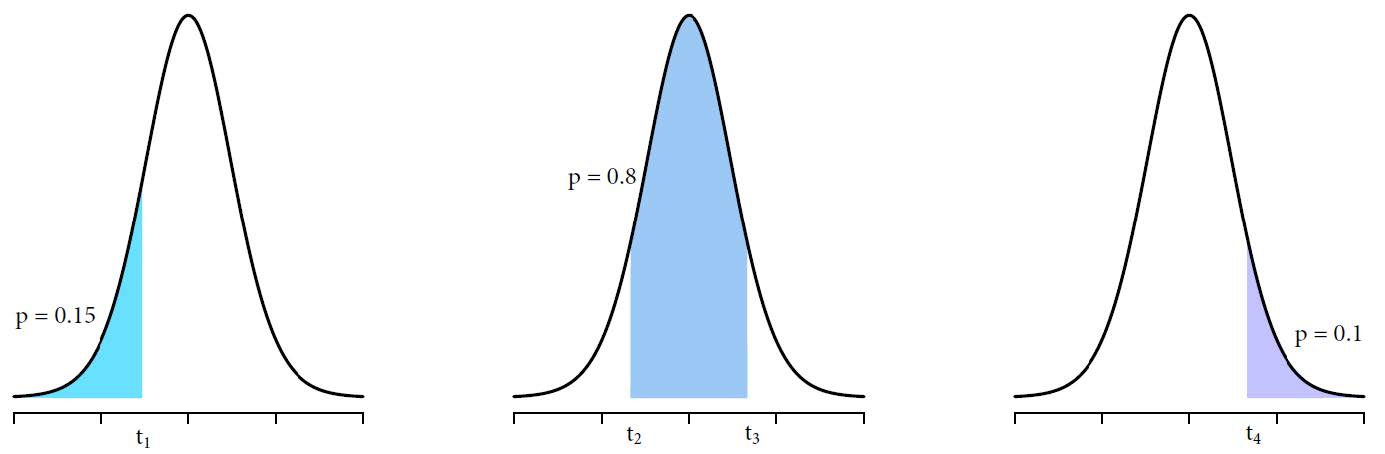
\includegraphics[width=\textwidth]{Files/Images/tdistributions2.jpg}
\end{center}

\question{
    For the situation where there are 19 \concepts{degrees of freedom}, use the \rcode{qt()} function to get the \concept{t-values} (t$_1$, t$_2$, t$_3$, t$_4$) for the three situations shown in the picture above.
}

\hint{For the picture on the right keep in mind that the \rcode{qt()} function by default returns the value for the left tail of the distribution.}

\rcodeanswermedium

\emptyanswerbox{
    t$_1$: \shortanswerline \hspace*{3cm} t$_2$: \shortanswerline
    \answerskip
    t$_3$: \shortanswerline \hspace*{3cm} t$_4$: \shortanswerline
}

\begin{center}
    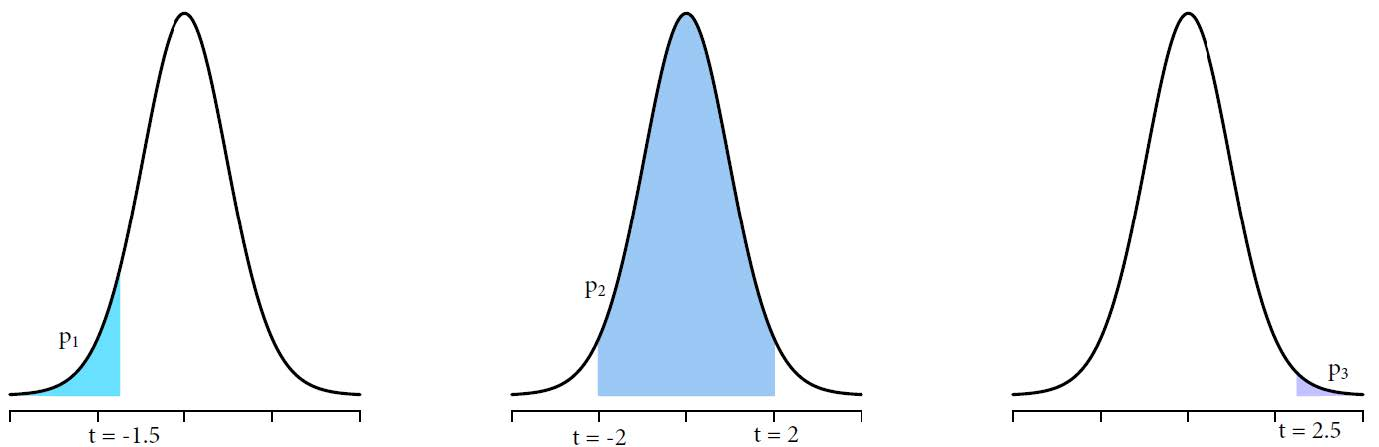
\includegraphics[width=\textwidth]{Files/Images/tdistributions3.jpg}
\end{center}

\clearpage % Page break

\question{
    For the situation where there are 11 \concept{degrees of freedom}, use the \rcode{pt()} function to get the probabilities p$_1$, p$_2$, and p$_3$ (area under the curve) for the three situations shown in the figures above.
}

\hint{For the picture in the middle and the right keep in mind that the \rcode{pt()} function by default uses the left tail and the total area under the curve is 1.}

\rcodeanswermedium

\emptyanswerbox{
    p$_1$: \tinyanswerline \hspace*{2cm} p$_2$: \tinyanswerline \hspace*{2cm} p$_3$: \tinyanswerline
}

When you test a value for a \concept{population mean}, there exist three types of tests: \\

\begin{minipage}[t]{0.33\textwidth}
Two-tailed inequality test: \\
\\
$H_0: \mu = \mu_0$ \\
$H_1: \mu \neq \mu_0$
\end{minipage}
\begin{minipage}[t]{0.33\textwidth}
One-tailed right sided test: \\
\\
$H_0: \mu \leq \mu_0$ \\
$H_1: \mu > \mu_0$
\end{minipage}
\begin{minipage}[t]{0.33\textwidth}
One-tailed left sided test: \\
\\
$H_0: \mu \geq \mu_0$ \\
$H_1: \mu < \mu_0$
\end{minipage}
\vspace*{0.5cm}

\question{
    Give a critical \concept{t-value} for the three tests described above using a confidence of 98\% and 28 \concept{degrees of freedom}.
}

\hint{Use the \rcode{qt()} function in \texttt{R}}.

\rcodeanswermedium

\emptyanswerbox{
    Two-tailed inequality test: \shortanswerline 
    \answerskip
    One-tailed right sided test: \hspace*{-5pt}\shortanswerline 
    \answerskip
    One-tailed left sided test: \shortanswerline 
}

\clearpage % Page break

Three $n = 29$ \concept{samples} were done on three different populations and the \concept{t-score} based on these \concept{samples} was calculated:

\begin{minipage}[t]{0.33\textwidth}
Two-tailed inequality test: \\
\\
$H_0: \mu = 50$ \\
$H_1: \mu \neq \50$ \\
\\
$t = 2.6$
\end{minipage}
\begin{minipage}[t]{0.33\textwidth}
One-tailed right sided test: \\
\\
$H_0: \mu \leq \50$ \\
$H_1: \mu > \50$ \\
\\
$t = -2.3$
\end{minipage}
\begin{minipage}[t]{0.33\textwidth}
One-tailed left sided test: \\
\\
$H_0: \mu \geq \50$ \\
$H_1: \mu < \50$ \\
\\
$t = 1.6$
\end{minipage}
\vspace*{0.5cm}

\question{
    Using a confidence of 98\%, find out whether the \concept{null hypothesis} $H_0$ is rejected for each of these three cases.
}

\hint{Use the \concept{critical t-values} from the previous assignment and compare these with the sample \concept{t-scores} to draw your conclusion for each of these outcomes.}

\emptyanswerbox{
    Two-tailed inequality test: \hspace*{1.5cm} \textbf{$H_0$ rejected} / \textbf{$H_0$ not rejected}
    \answerbreak
    Explanation: \rule{.75\textwidth}{0.4pt}
    \answerskip
    \answerskip
    One-tailed right sided test: \hspace*{-5pt}\hspace*{1.5cm} \textbf{$H_0$ rejected} / \textbf{$H_0$ not rejected}
    \answerbreak
    Explanation: \rule{.75\textwidth}{0.4pt}
    \answerskip
    \answerskip
    One-tailed left sided test: \hspace*{1.5cm} \textbf{$H_0$ rejected} / \textbf{$H_0$ not rejected}
    \answerbreak
    Explanation: \rule{.75\textwidth}{0.4pt}    
}

\clearpage % Page break